\section{Synchronisation variable}

Comme vus dans la partie précédente, le partage des données dans le cas des processus ainsi que des threads et très différents. D'un cote nous avons les processus, qui, suite à l'appel de fonction \textit{fork()}, ne partagerons pas de données entre les deux processus ce qui rends presque impossible tout communication entre ceux-ci. Pour remédier au problème de manque de communication inter-processus, nous avons à notre disposition plusieurs outils tels que les pipes ou l'espace mémoire partagée. Mais attention, il faudras dès lors gérer la concurrence d'accès à ces données en utilisant par exemple des sémaphore, de verrous de fichiers, etc... Comme nous pouvons le constater, rendre possible la communication inter-processus est un procédé assez coûteux en performances. Copier tout un processus avec tout son contexte, ensuite créer un moyen de communication (pipe, mémoire partagée, etc...) et pour finir, il faut mettre en place un système de gestion de concurrence d'accès à ces données (sémaphore, verrous de fichier, etc ...).
\\

De l'autre cote, les threads vont partager un grands nombre de données entre eux. Ce qui est très intéressant lorsque nous voulons faire communiquer les processus entre eux. Mais advient alors une autre problématique : gérer la concurrence d'accès aux-dites données. Nous pourrions utiliser alors unes des solutions énoncée juste avant pour les processus, mais leurs utilisations est limité à de rare cas car ces solutions sont soit plus difficiles à mettre en place, soit plus coûteuses en performances. C'est à cet effet la que la librairie \textit{pthread} mets à notre disposition les \textbf{mutex}.

\subsection{Les mutex}
Un \textbf{mutex} (abréviation de "mutual exclusion", en français "exclusion mutuelle") est un mécanisme de synchronisation utilisé pour garantir qu'un seul thread à la fois peut accéder à une ressource partagée ou une section critique du code. L'objectif principal d'un \textbf{mutex} est d'éviter les conflits d'accès concurrents qui pourraient conduire à des résultats indéterminés ou incorrects dans un programme multithread.

En d'autres termes, un \textbf{mutex} agit comme un verrou que les threads doivent acquérir avant d'entrer dans une zone critique du code. S'il est déjà détenu par un thread, les autres threads qui tentent de le verrouiller doivent attendre jusqu'à ce qu'il soit libéré.

Un \textbf{mutex} offre deux opérations principales :
\\
\begin{itemize}
    \item Verrouillage (Locking) : Un thread qui souhaite accéder à la section critique commence par verrouiller le mutex. Si le mutex est libre, le thread l'acquiert et continue. Si le mutex est déjà verrouillé par un autre thread, le thread actuel est mis en attente jusqu'à ce que le mutex soit libéré.
\\
    \item Déverrouillage (Unlocking) : Une fois qu'un thread a terminé ses opérations dans la section critique, il déverrouille le mutex, permettant ainsi à d'autres threads en attente d'acquérir le mutex et accéder à la section critique à leur tour.
\end{itemize}
\vspace{\baselineskip}

\begin{lstlisting}[title = Code sans mutex]
#include <pthread.h>
#include <stdio.h>


static int glob = 0;
static void *
routine(void *arg)
{

int loc, j;
for (j = 0; j <100000000 ; j++) {
loc = glob;
loc++;
glob = loc;
}
return NULL;
}
int
main(int argc, char *argv[])
{
pthread_t t1, t2;

if (pthread_create(&t1, NULL, &routine, NULL))
	{
		return 1;
	}
	if (pthread_create(&t2, NULL, &routine, NULL))
	{
		return 2;
	}

	if (pthread_join(t1, NULL))
	{
		return 3;
	}
	if (pthread_join(t2, NULL))
	{
		return 4;
	}

	printf("Valeur de la variable globale : %d \n", glob);



}

\end{lstlisting}
\vspace{\baselineskip}

La valeur de la variable globale seras alors différente à chaque exécution de code : 
\\
\line(1,0){\linewidth}
\\
Première exécution : 114300045\\
Deuxième execution : 118548239
\\
\line(1,0){\linewidth}

\begin{lstlisting}[title = Utilisation mutex]
#include <pthread.h>
#include <stdio.h>


static int glob = 0;
pthread_mutex_t mutex = PTHREAD_MUTEX_INITIALIZER;
static void *
routine(void *arg)
{
    pthread_mutex_lock(&mutex);
int loc, j;
for (j = 0; j <100000000 ; j++) {
loc = glob;
loc++;
glob = loc;
}
pthread_mutex_unlock(&mutex);
return NULL;
}
int
main(int argc, char *argv[])
{
pthread_t t1, t2;

if (pthread_create(&t1, NULL, &routine, NULL))
	{
		return 1;
	}
	if (pthread_create(&t2, NULL, &routine, NULL))
	{
		return 2;
	}

	if (pthread_join(t1, NULL))
	{
		return 3;
	}
	if (pthread_join(t2, NULL))
	{
		return 4;
	}

	printf("Valeur de la variable globale : %d\n", glob);



}
\end{lstlisting}
\vspace{\baselineskip}

Or, grâce à l'utilisation d'un \textbf{mutex}, la valeur de la variable globale seras toujours égale à 200000000.

\subsubsection{Les mutex statiques}

Au sein de la libraire \textit{pthread}, nous avons à notre dispositions 2 types de \textbf{mutex}. Les mutex statiques ainsi que les mutex dynamiques. Commençons par les mutex les plus simples, les mutex statiques.
Les mutex statiques sont les mutex les plus simples d'utilisation. l'initialisation d'un mutex statique est très simple. Son initialisation est effectuée statiquement lors de la compilation, ce qui signifie que son cycle de vie est lié au cycle de vie du programme. On initialise un mutex statique comme suit : 
\\ 

\begin{lstlisting}[title = Initialisation mutex statique]
#include <pthread.h>
    pthread_mutex_t mutex = PTHREAD_MUTEX_INITIALIZER;
\end{lstlisting}
\vspace{\baselineskip}

L'initialisation statique signifie que le mutex est prêt à être utilisé dès le début du programme. Cela signifie également qu'il n'y as pas besoin de détruire manuellement le mutex quand on en as plus besoin car son cycle de vie est lié à celui du programme, et il est généralement utilisé jusqu'à la fin de l'exécution du programme. Le mutex statique se caractérise principalement par :
\\
\begin{itemize}
    \item Initialisation Automatique : Le mutex est initialisé automatiquement lors de la compilation avec une valeur initiale qui le rend utilisable sans appel explicite à une fonction d'initialisation.
    \\
    \item Portée Locale ou Globale : Un mutex statique peut être déclaré à l'intérieur d'une fonction pour une portée locale, ou en dehors de toute fonction pour une portée globale.
    \\
    \item Durée de Vie Liée au Programme : Un mutex statique existe pendant toute la durée d'exécution du programme. Il est généralement utilisé pour des sections critiques partagées entre plusieurs threads.
    \\
    \item Utilisation avec \textit{pthread\_mutex\_lock} et \textit{pthread\_mutex\_unlock} : On peut utiliser les fonctions \textit{pthread\_mutex\_lock} et \textit{pthread\_mutex\_unlock} pour verrouiller et déverrouiller le mutex respectivement.
\end{itemize}
\vspace{\baselineskip}

Afin de bien visualiser le fonctionnement du mutex statique, nous pouvons retourner au code juste au-dessus où la synchronisation de l'incrémentation de la variable globale se fait grâce à un mutex statique.

\subsubsection{Les mutex dynamiques}

Au contraire du mutex statique, le mutex dynamique est bien plus complexe à mettre en place. Un mutex dynamique est un mutex dont l'initialisation est effectuée dynamiquement pendant l'exécution du programme. Contrairement à un mutex statique qui est initialisé statiquement lors de la compilation, un mutex dynamique est généralement alloué sur le tas (heap) à l'aide de fonctions spécifiques. Afin d'utiliser un mutex dynamique, il nous faut 2 fonctions :
\\ 
\begin{itemize}
    \item La fonction d'initialisation : 
    \begin{lstlisting}[title = Initialisation mutex dynamique]
    #include <pthread.h>
        int pthread_mutex_init(pthread_mutex_t *mutex, const pthread_mutexattr_t *attr);
    \end{lstlisting}
    \vspace{\baselineskip}
    \item La fonction de destruction : 
    \begin{lstlisting}[title = Destruction mutex dynamique]
    #include <pthread.h>
        int pthread_mutex_destroy(pthread_mutex_t *mutex);
    \end{lstlisting}    
\end{itemize}
\vspace{\baselineskip}

Maintenant que nous savons comment initialiser et détruire un mutex dynamique, regardons ce que cela donne en pratique : 
\vspace{\baselineskip}
\begin{lstlisting}[title = Code mutex dynamique]
#include <pthread.h>
#include <stdio.h>

struct SharedData {
    int glob;
    pthread_mutex_t mutex;
};

static void *routine(void *arg) {
    struct SharedData *donnees = (struct SharedData *)arg;
    pthread_mutex_lock(&(donnees->mutex));
    int loc, j;
    for (j = 0; j < 1000000; j++) {
        loc = donnees->glob;
        loc++;
        donnees->glob = loc;
    }
    pthread_mutex_unlock(&(donnees->mutex));
    return NULL;
}

int main(int argc, char *argv[]) {
    pthread_t t1, t2;
    struct SharedData donnees;
    donnees.glob = 0;

    // Initialisation du mutex
    if (pthread_mutex_init(&(donnees.mutex), NULL) != 0) {
        fprintf(stderr, "Erreur lors de l'initialisation du mutex\n");
        return 1;
    }

    if (pthread_create(&t1, NULL, &routine, (void *)&donnees)) {
        fprintf(stderr, "Erreur lors de la creation du thread 1\n");
        return 2;
    }
    if (pthread_create(&t2, NULL, &routine, (void *)&donnees)) {
        fprintf(stderr, "Erreur lors de la creation du thread 2\n");
        return 3;
    }

    if (pthread_join(t1, NULL)) {
        fprintf(stderr, "Erreur lors de l'attente du thread 1\n");
        return 4;
    }
    if (pthread_join(t2, NULL)) {
        fprintf(stderr, "Erreur lors de l'attente du thread 2\n");
        return 5;
    }

    printf("Valeur de la variable globale : %d\n", donnees.glob);

    // Destruction du mutex
    if (pthread_mutex_destroy(&(donnees.mutex)) != 0) {
        fprintf(stderr, "Erreur lors de la destruction du mutex\n");
        return 6;
    }

    return 0;
}


\end{lstlisting}   
\vspace{\baselineskip}

A la fin de l'exécution de ce programme, on verras le message suivant : 
\\
\line(1,0){\linewidth}
\\
Valeur de la variable globale : 2000000
\\
\line(1,0){\linewidth}

\subsubsection{Le choix de mutex}


Maintenant viens alors la question suivante, quand utiliser quel type de mutex? Le choix entre un mutex statique et dynamique dépend des besoins spécifiques de notre programme et de la portée que nous souhaitons donner au mutex. Voici quelques points à considérer pour nous aider à décider entre un mutex statique et dynamique :
\vspace{\baselineskip}
\begin{itemize}
    \item Portée du Mutex :
    \begin{itemize}
    \vspace{\baselineskip}
        \item Mutex Statique : Si le mutex est destiné à être utilisé à l'intérieur d'une seule fonction ou d'un seul fichier, un mutex statique peut être approprié.
        \\
        \item Mutex Dynamique : Si le mutex doit être partagé entre plusieurs fichiers ou doit être accessible à partir de plusieurs parties du programme, un mutex dynamique pourrait être plus approprié.
    \end{itemize}
\vspace{\baselineskip}
    \item Durée de Vie du Mutex :
    \vspace{\baselineskip}
    \begin{itemize}
        \item Mutex Statique : La durée de vie d'un mutex statique est la durée d'exécution du programme. Il est créé une seule fois lors de l'exécution du programme et persiste jusqu'à la fin.
        \\ 
        \item Mutex Dynamique : Un mutex dynamique peut être alloué et libéré dynamiquement pendant l'exécution du programme. Si nous avons besoin de créer et de détruire des mutex de manière dynamique, l'utilisation d'un mutex dynamique est plus judicieuse.
    \end{itemize}
\vspace{\baselineskip}
    \item Flexibilité :
    \vspace{\baselineskip}
    \begin{itemize}
        \item Mutex Statique : Les mutex statiques sont définis au moment de la compilation et ne peuvent pas être créés ou détruits dynamiquement pendant l'exécution. Ils offrent une utilisation simple mais moins de flexibilité.
        \\
        \item Mutex Dynamique : Les mutex dynamiques peuvent être alloués et libérés dynamiquement pendant l'exécution, ce qui offre une plus grande flexibilité.
    \end{itemize}
\vspace{\baselineskip}
    \item Complexité :
    \vspace{\baselineskip}
    \begin{itemize}
        \item Mutex Statique : Les mutex statiques sont généralement plus simples à utiliser car ils sont définis statiquement au niveau du code.
        \\
        \item Mutex Dynamique : Les mutex dynamiques nécessitent une allocation et une libération explicites, ce qui peut ajouter une complexité supplémentaire.
    \end{itemize}
\end{itemize}
\vspace{\baselineskip}

En bref, si nous avons besoin d'un mutex pour synchroniser une petite variable ou zone critique au sein d'un même processus, il est alors préférable d'utiliser un mutex statique au vus de sa simplicité et rapidité. Pour tout autre usage plus complexe, il est avisé d'utiliser un mutex dynamiques.





\subsection{Mutex conditionnel}

Il est bon de savoir qu'il existe la possibilité d'adapter le fonctionnement d'un mutex à des besoins plus spécifiques. Un exemple intéressant est le mutex conditionnel.Un mutex conditionnel, est un mécanisme de synchronisation avancé utilisé dans les systèmes multi-threads pour permettre à des threads de coopérer en fonction de certaines conditions. Il s'agit généralement d'une combinaison d'un mutex et d'une variable de condition.
\\


Voici une description des composants d'un mutex conditionnel :
\vspace{\baselineskip}
\begin{itemize}
    \item Mutex : Un mutex conditionnel utilise un mutex pour garantir un accès exclusif à une ressource partagée.
    \\
    \item Variable de condition : 
    \vspace{\baselineskip}
    \begin{itemize}
        \item Une variable de condition est utilisée pour signaler ou attendre une condition spécifique. Elle est généralement associée à un mutex pour assurer une synchronisation correcte.
        \\
        \item Un thread peut signaler la condition à d'autres threads lorsqu'il effectue une action importante, et d'autres threads peuvent attendre que la condition soit satisfaite avant de continuer leur exécution.
    \end{itemize}
\end{itemize}
\vspace{\baselineskip}

Afin d'utiliser les threads conditionnel, nous avons des fonctions mises à notre disposition par la librairie \textit{pthread}. 
\vspace{\baselineskip}
\begin{itemize}
    \item \textbf{pthread\_cond\_init} : 
    \vspace{\baselineskip}
    \begin{lstlisting}[title = Initialisation mutex conditionnel]
    #include <pthread.h>
        int pthread_cond_init(pthread_cond_t *cond, const pthread_condattr_t *attr);
    \end{lstlisting}
    
    La fonction \textit{pthread\_cond\_init} initialise la variable de condition spécifiée par cond. Après son appel, la variable de condition est prête à être utilisée avec d'autres fonctions de l'API POSIX pour la synchronisation entre threads.
    \\
    \item \textbf{pthread\_cond\_wait} : 
    \vspace{\baselineskip}
    \begin{lstlisting}[title = Wait mutex conditionel]
#include <pthread.h>
    int pthread_cond_wait(pthread_cond_t *cond, pthread_mutex_t *mutex);
    \end{lstlisting}

    Elle est utilisée pour faire attendre un thread jusqu'à ce qu'une condition spécifique soit satisfaite. La fonction \textit{pthread\_cond\_wait} doit être utilisée en conjonction avec un mutex.
    \\
    \item \textbf{pthread\_cond\_signal} : 
    \vspace{\baselineskip}
    \begin{lstlisting}[title = Signal mutex conditionnel]
#include <pthread.h>
    int pthread_cond_signal(pthread_cond_t *cond);
    \end{lstlisting}

    La fonction \textit{pthread\_cond\_signal} permet de signaler (ou réveiller) un thread en attente sur une variable de condition. Lorsqu'un thread exécute \textit{pthread\_cond\_signal} sur une variable de condition, il indique à un thread en attente sur cette condition qu'il peut reprendre l'exécution. Cependant, cela ne garantit pas que le thread réveillé prendra immédiatement la main ; cela dépend de l'ordonnanceur.
     \vspace{\baselineskip}
    \item \textbf{pthread\_cond\_broadcast} : 
    \vspace{\baselineskip}
    \begin{lstlisting}[title = Broadcast mutex conditionnel]
#include <pthread.h>
    int pthread_cond_broadcast(pthread_cond_t *cond);
    \end{lstlisting}

    La fonction \textit{pthread\_cond\_broadcast} délivre un signal à tous les threads en attente sur la variable de condition spécifiée. Cela signifie que tous les threads qui étaient bloqués en attente sur cette condition seront réveillés simultanément.
\end{itemize}
 \vspace{\baselineskip}

Les mutex conditionnel sont bien évidemment utilisé avec les fonctions de bases des mutex ; \textit{pthread\_mutex\_init}, \textit{pthread\_mutex\_lock}, et \textit{pthread\_mutex\_unlock}.

Maintenant pour mettre tout ce que nous avons vus en pratique, afin de bien visualiser, voici un petit code d'exemple :
\vspace{\baselineskip}
\begin{lstlisting}[title = Code mutex conditionnel]
#include <pthread.h>
#include <stdio.h>
#include <string.h>

char ressource_partagee[] = "texte";
int condition = 0;
pthread_mutex_t mutex = PTHREAD_MUTEX_INITIALIZER;
pthread_cond_t cond = PTHREAD_COND_INITIALIZER;

void *routine1(void *arg) {
    pthread_mutex_lock(&mutex);
    char str[7] = "thread1";
    condition = 1;
    strcat(ressource_partagee, str);
    pthread_cond_signal(&cond);
    pthread_mutex_unlock(&mutex);

    return NULL;
}

void *routine2(void *arg) {
    pthread_mutex_lock(&mutex);
    while (condition != 1) {
        pthread_cond_wait(&cond, &mutex);
    }

    printf("J'ai lu %s\n", ressource_partagee);

    pthread_mutex_unlock(&mutex);

    return NULL;
}

int main() {
    pthread_t t1, t2;

    if (pthread_create(&t2, NULL, &routine2, NULL)) {
        return 2;
    }

    sleep(5);

    if (pthread_create(&t1, NULL, &routine1, NULL)) {
        return 1;
    }

    if (pthread_join(t1, NULL)) {
        return 3;
    }
    if (pthread_join(t2, NULL)) {
        return 4;
    }

    return 0;
}

\end{lstlisting}



Pour bien résumé le fonctionnement typique d'un mutex conditionnel, comme vus dans le code ci dessus, nous avons les étapes suivantes :
\vspace{\baselineskip}
\begin{itemize}
    \item Un thread acquiert le mutex avant de vérifier une condition. Si la condition n'est pas satisfaite, le thread libère le mutex et s'endort sur la variable de condition.
    \\
    \item Un autre thread effectue une action importante, modifie la condition, acquiert le mutex, et signale à la variable de condition que la condition a été modifiée.
    \\
    \item Le premier thread, qui était en attente, est réveillé par le signal et réacquiert le mutex. Il révérifie la condition et peut continuer son exécution si la condition est maintenant satisfaite.
\end{itemize}
\vspace{\baselineskip}

\subsubsection{Remarques}

Comme on peut le voir dans le code, la fonction \textit{pthread\_cond\_wait()} est entourée d'un while. Même si la fonction en elle même vas attendre un signal de la condition, ceci représente néanmoins une bonne pratique de codage car elle permet d'éviter faux réveils.
\vspace{\baselineskip}

Il est également intéressant d'attirer l'attention sur l'odre dans lequel on signale et on débloque le mutex dans la fonction \textit{routine1}. Comme nous pouvons le constater dans cette fonction, on signale d'abord via la condition que le mutex est libre et par la suite on le libère réellement. Cela semble contre intuitif! Pourquoi d'abord signaler la libération avant même de libérer? L'ordre dans \textit{routine1} (signal d'abord, puis déverrouillage) est couramment utilisé dans le modèle \textbf{signal and wait} (signaler et attendre). Voici pourquoi cet ordre est généralement préféré : 

\begin{itemize}
    \item \textbf{Éviter les faux réveils} : La fonction \textit{pthread\_cond\_wait()} peut parfois se réveiller sans qu'aucun signal ne soit émis. C'est ce qu'on appelle un "faux réveil". En émettant le signal avant de déverrouiller le mutex, on s'assure que le signal est déjà émis lorsque le thread se réveille, évitant ainsi d'entrer dans la section critique sans raison. 
\\
    \item \textbf{Éviter les courses critiques} : Si le déverrouillage du mutex était effectué avant l'émission du signal, il existerait une fenêtre de temps pendant laquelle le mutex est déverrouillé mais le signal n'a pas encore été émis. Dans ce laps de temps, un autre thread pourrait acquérir le mutex et modifier la condition, créant une course critique.
\end{itemize}

\subsection{Deadlock}

Lors de l'utilisation des mutex, il faut faire très attentions à ne pas provoquer un \textit{deadlock}. Un \textit{deadlock} est une situation dans laquelle deux ou plusieurs processus ou threads sont incapables de progresser parce que chacun d'entre eux attend quelque chose que l'autre a. En d'autres termes, chaque processus ou thread détient des ressources et attend d'en acquérir d'autres, créant ainsi un cercle d'attente mutuelle.
Voici un exemple simple illustrant un deadlock :
\begin{mdframed}    
Processus A détient la ressource 1 et demande la ressource 2.\\
\\
Processus B détient la ressource 2 et demande la ressource 1.
\end{mdframed}
Dans cette situation, chaque processus détient une ressource et attend l'autre pour pouvoir progresser. Ainsi, un deadlock se produit.Les deadlocks sont des situations indésirables car elles peuvent entraîner une impasse complète dans l'exécution du programme, nécessitant une intervention extérieure pour résoudre le problème. 
\vspace{\baselineskip}
\begin{lstlisting}[title = Code deadlock]
#include <pthread.h>
#include <stdio.h>

pthread_mutex_t mutex1 = PTHREAD_MUTEX_INITIALIZER;
pthread_mutex_t mutex2 = PTHREAD_MUTEX_INITIALIZER;

void *routine1(void *arg) {
    printf("Thread 1 : Attente de mutex1\n");
    pthread_mutex_lock(&mutex1);

    printf("Thread 1 : Verrouillage de mutex1\n");
    
    sleep(1);

    printf("Thread 1 : Attente de mutex2\n");
    pthread_mutex_lock(&mutex2);



    pthread_mutex_unlock(&mutex2);
    pthread_mutex_unlock(&mutex1);

    return NULL;
}

void *routine2(void *arg) {
    printf("Thread 2 : Attente de mutex2\n");
    pthread_mutex_lock(&mutex2);

    printf("Thread 2 : Verrouillage de mutex2\n");

    sleep(1);

    printf("Thread 2 : Attente de mutex1\n");
    pthread_mutex_lock(&mutex1);



    pthread_mutex_unlock(&mutex1);
    pthread_mutex_unlock(&mutex2);

    return NULL;
}

int main() {
    pthread_t thread1, thread2;


    pthread_create(&thread1, NULL, routine1, NULL);
    pthread_create(&thread2, NULL, routine2, NULL);


    pthread_join(thread1, NULL);
    pthread_join(thread2, NULL);

    return 0;
}
\end{lstlisting}   
\vspace{\baselineskip}

\begin{figure}[ht]
    \centering
    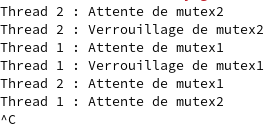
\includegraphics[width=0.8\linewidth]{deadlock.png}
    \caption{résultat deadlock}
    \label{fig:result_deadlock}
\end{figure}

\subsection{Remarques}

La question de la synchronisation de concurrence est un sujet très complexe dont de nombreux spécialiste on passer un temps incalculable afin de trouver la meilleure solution, le meilleur algorithme pour rendre ce processus le plus performant possible. Tout ces système de gestion de concurrence peuvent être plus ou moins utilisable dans le cas des threads et des processus. Par exemple, on peut tout à fait utiliser des sémaphores ou des verrous de fichiers dans un thread. Certains sont plus adapté à un cas où un autre. Par exemple, il est techniquement possible d'utiliser des mutex avec un processus \textit{forké}, mais cette implémentation est bien trop complexe pour qu'elle n'aie une utilisation censée. 


